% !TEX TS-program = xelatex
% !TEX encoding = UTF-8 Unicode
% -*- coding: UTF-8; -*-
% vim: set fenc=utf-8

%%%%%%%%%%%%%%%%%%%%%%%%%%%%%%%%%%%%%%%%%%%%%%%%%%%%%%%%%%%%%%%%%
%% Thesis.tex
%% <https://github.com/zachscrivena/simple-thesis-dissertation>
%% This is free and unencumbered software released into the
%% public domain; see <http://unlicense.org> for details.
%%%%%%%%%%%%%%%%%%%%%%%%%%%%%%%%%%%%%%%%%%%%%%%%%%%%%%%%%%%%%%%%%

% See "README.md" for instructions on compiling this document.

\documentclass[letterpaper,nonstopmode,draftmode,msfonts]{gvsuthesis}
% Class options:
% [a4paper, letterpaper]
% nonstopmode
% draftmode
% [*doublespacing*, singlespacing, onehalfspacing]
% msfonts
% sansfonts

%%%%%%%%%%%%%%%%%%%%%%%%%%%%%%%%%%%%%%%%%%%%%%%%%%%%%%%%%%%%%%%%%
%%                                                      PREAMBLE
%%%%%%%%%%%%%%%%%%%%%%%%%%%%%%%%%%%%%%%%%%%%%%%%%%%%%%%%%%%%%%%%%

% Packages
\usepackage{pdftexcmds}

% Setup bools (\ifBoolName ... \fi)
\newbool{HasListOfTables}
\newbool{HasListOfFigures}
\newbool{HasCurriculumVitae}

% Document properties
\def\DocumentTitle{Your Thesis Title}
\def\AuthorName{Firstname Lastname}
\def\AuthorFullName{Firstname Middlename Lastname}
\def\Degree{Master of Science}
\def\AcademicUnit{Computer Information Systems}
\def\Year{2020}
\def\Month{December}

% PDF settings and properties
\hypersetup{
pdftitle={\DocumentTitle},
pdfauthor={\AuthorName},
pdfsubject={Master's Thesis, Grand Valley State University, 2020},
pdfcreator={XeLaTeX},
pdfproducer={},
pdfkeywords={},
unicode=true,
bookmarks=true,
bookmarksopen=true,
pdfstartview=FitH,
pdfpagelayout=OneColumn,
pdfpagemode=UseOutlines,
hidelinks,
breaklinks,
bookmarksnumbered}
\pagestyle{plain}

% Macros
%%%%%%%%%%%%%%%%%%%%%%%%%%%%%%%%%%%%%%%%%%%%%%%%%%%%%%%%%%%%%%%%%%%%%%%%%%%%%%%%%
% vvv These macros are only for the example content, and can be deleted vvv %%%%%
%%%%%%%%%%%%%%%%%%%%%%%%%%%%%%%%%%%%%%%%%%%%%%%%%%%%%%%%%%%%%%%%%%%%%%%%%%%%%%%%%
\DeclareMathOperator*{\argmax}{arg\,max}
\DeclareMathOperator*{\argmin}{arg\,min}
\renewcommand{\binom}[2]{\left(\genfrac{}{}{0pt}{}{#1}{#2}\right)}
\newcommand{\ceil}[1]{{\left\lceil{#1}\right\rceil}}
\newcommand{\floor}[1]{{\left\lfloor{#1}\right\rfloor}}
\DeclareMathOperator{\lcm}{lcm}
\newcommand{\ZZ}{{\mathbb{Z}}}
%%%%%%%%%%%%%%%%%%%%%%%%%%%%%%%%%%%%%%%%%%%%%%%%%%%%%%%%%%%%%%%%%%%%%%%%%%%%%%%%%
% ^^^ These macros are only for the example content, and can be deleted ^^^ %%%%%
%%%%%%%%%%%%%%%%%%%%%%%%%%%%%%%%%%%%%%%%%%%%%%%%%%%%%%%%%%%%%%%%%%%%%%%%%%%%%%%%%

%%%%%%%%%%%%%%%%%%%%%%%%%%%%%%%%%%%%%%%%%%%%%%%%%%%%%%%%%%%%%%%%%
%%                                                TEMPLATE SETUP
%%%%%%%%%%%%%%%%%%%%%%%%%%%%%%%%%%%%%%%%%%%%%%%%%%%%%%%%%%%%%%%%%

% If not using, leave blank.
\def\Dedication{For Kramer, my loyal fish.}
\def\Acknowledgements{I'd like to thank my advisors.}
\def\Preface{}
\def\Abstract{This is a thesis abstract.}

% If not using, comment out
\booltrue{HasListOfTables}
\booltrue{HasListOfFigures}
\booltrue{HasCurriculumVitae}

%%%%%%%%%%%%%%%%%%%%%%%%%%%%%%%%%%%%%%%%%%%%%%%%%%%%%%%%%%%%%%%%%
%%                                               ACTUAL DOCUMENT
%%%%%%%%%%%%%%%%%%%%%%%%%%%%%%%%%%%%%%%%%%%%%%%%%%%%%%%%%%%%%%%%%

\begin{document}

% Front-matter:
%   Title page
%   Approval page
%   Dedication
%   Acknowledgements
%   Preface
%   Abstract
%   TOCs
% Use Roman numerals (i, ii, iii, etc.) for page numbers in the front matter.
\pagenumbering{roman}

%%%%%%%%%%%%%%%%%%%%%%%%%%%%%%%%%%%%%%%%%%%%%%%%%%%%%%%%%%%%%%%%%
%% TITLE PAGE.
%%%%%%%%%%%%%%%%%%%%%%%%%%%%%%%%%%%%%%%%%%%%%%%%%%%%%%%%%%%%%%%%%

% No headers or footers on the title page.
\thispagestyle{empty}

\begingroup
\centering
\setstretch{1.0}
~
\\[1em]
\sffamily\bfseries\fontsize{26}{31.2}\selectfont
\DocumentTitle
\\
Use Manual Line Breaks If Necessary
\\[0.4in]
\normalfont\large
Thesis by
\\[0.25em]
\sffamily\bfseries\Large
\AuthorName
\\[0.4in]
\normalfont\normalsize
In Partial Fulfillment of the Requirements
\\[0.5em]
for the Degree of
\\[0.5em]
Doctor of Philosophy
\\[0.5em]
in
\\[0.5em]
Electrical Engineering and Computer Science
\vfill
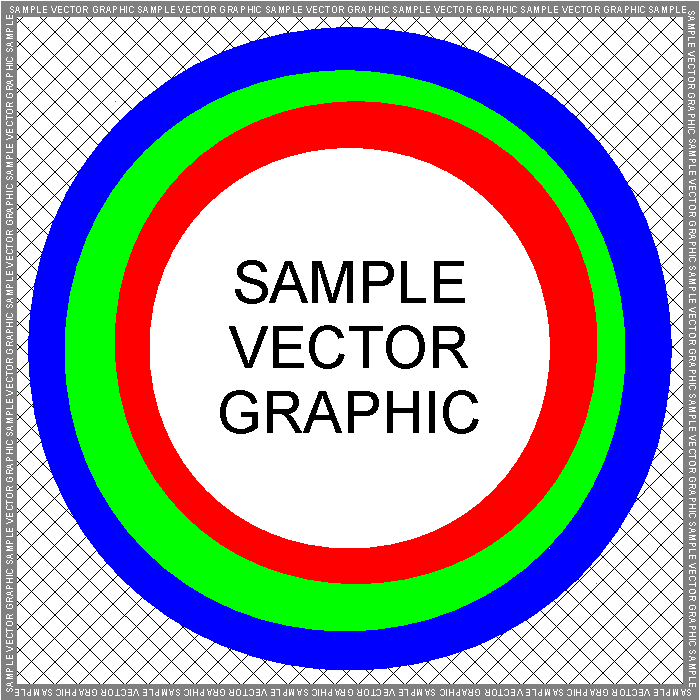
\includegraphics[height=1.8in]
{Figures/Figure-SchoolLogo}
\\[1.5em]
University Institute of College
\\[0.5em]
Springfield, New York, USA
\\[1.5em]
2016
\\[0.5em]
(Defended November 25, 2016)
\par
\endgroup

\clearpage

%%%%%%%%%%%%%%%%%%%%%%%%%%%%%%%%%%%%%%%%%%%%%%%%%%%%%%%%%%%%%%%%%
%% COPYRIGHT PAGE.
%%%%%%%%%%%%%%%%%%%%%%%%%%%%%%%%%%%%%%%%%%%%%%%%%%%%%%%%%%%%%%%%%

\pagestyle{plain}
\setcounter{page}{2}

\begingroup
\centering
\setstretch{1.0}
\null
\vfill
{\sffamily\textcopyright}~2016
\\[0.5em]
\AuthorName
\\[0.5em]
All Rights Reserved
\par
\endgroup

\clearpage

%%%%%%%%%%%%%%%%%%%%%%%%%%%%%%%%%%%%%%%%%%%%%%%%%%%%%%%%%%%%%%%%%
%% DEDICATION PAGE.
%%%%%%%%%%%%%%%%%%%%%%%%%%%%%%%%%%%%%%%%%%%%%%%%%%%%%%%%%%%%%%%%%

\begingroup
\centering
\setstretch{1.0}
~
\\[1in]
\textit{Insert dedication here}
\par
\endgroup

\clearpage

%%%%%%%%%%%%%%%%%%%%%%%%%%%%%%%%%%%%%%%%%%%%%%%%%%%%%%%%%%%%%%%%%
%% ACKNOWLEDGMENTS.
%%%%%%%%%%%%%%%%%%%%%%%%%%%%%%%%%%%%%%%%%%%%%%%%%%%%%%%%%%%%%%%%%

\chapter*{Acknowledgments}
\addcontentsline{toc}{chapter}{Acknowledgments}

{\color{red}%
Insert thesis acknowledgments here.
Thesis acknowledgments typically include research advisers and mentors, thesis committee members, collaborators, and funding sources.}

\lipsum[1-2]

\clearpage

%%%%%%%%%%%%%%%%%%%%%%%%%%%%%%%%%%%%%%%%%%%%%%%%%%%%%%%%%%%%%%%%%
%% ABSTRACT.
%%%%%%%%%%%%%%%%%%%%%%%%%%%%%%%%%%%%%%%%%%%%%%%%%%%%%%%%%%%%%%%%%

\chapter*{Abstract}
\addcontentsline{toc}{chapter}{Abstract}

{\color{red}%
Insert thesis abstract here.
The thesis abstract provides a concise description of the main contributions in the thesis.
Abstracting and indexing services usually include the thesis abstract in the catalog presented to users.
A well-written abstract could improve the chances of your work being discovered and cited by others in the research community.
The abstract should be self-contained (avoid citations and cross references) and should contain only plain text (avoid complicated mathematical expressions).}

\lipsum[1-6]

\clearpage

%%%%%%%%%%%%%%%%%%%%%%%%%%%%%%%%%%%%%%%%%%%%%%%%%%%%%%%%%%%%%%%%%
%% TABLE OF CONTENTS (TOC), LISTS OF FIGURES, TABLES, ETC.
%%%%%%%%%%%%%%%%%%%%%%%%%%%%%%%%%%%%%%%%%%%%%%%%%%%%%%%%%%%%%%%%%

\tableofcontents

\listoffigures

\listoftables

\clearpage

% Use Arabic numerals (1, 2, 3, etc.) for subsequent page numbers.
\pagenumbering{arabic}


% Thesis chapters
\chapter{Introduction}

{\color{red}%
Insert thesis introduction here.
This is a template for a simple thesis or dissertation (Ph.D. or master's degree) or technical report, in {\XeLaTeX}.
For more information, please visit
\begingroup
\par\centering
\href{https://github.com/zachscrivena/simple-thesis-dissertation}
{\url{https://github.com/zachscrivena/simple-thesis-dissertation}}
\par
\endgroup
}

\lipsum[1-8]


\chapter{Insert Chapter Title Here}
\label{Section:ChapAbbr}

\BlankFootnote{Insert chapter footnote here.
The chapter footnote could include citations to related publications by the author (``The material in this chapter was presented in part in ....'').}

%%%%%%%%%%%%%%%%%%%%%%%%%%%%%%%%%%%%%%%%%%%%%%%%%%%%%%%%%%%%%%%%%
%%%%%%%%%%%%%%%%%%%%%%%%%%%%%%%%%%%%%%%%%%%%%%%%%%%%%%%%%%%%%%%%%
%%%%%%%%%%%%%%%%%%%%%%%%%%%%%%%%%%%%%%%%%%%%%%%%%%%%%%%%%%%%%%%%%

\section{Introduction}
\label{Section:ChapAbbr:Introduction}

Insert chapter introduction here.
\lipsum[1-2]

\mbox{\textit{Related Work:}}
Our work is related to \cite{Examples:Conference01, Examples:Journal01, Examples:Conference02, Examples:Journal02, Examples:Conference03}.
\lipsum[3-4]

\mbox{\textit{Our Contribution:}}
\lipsum[5-6]

Proofs of theorems are deferred to \Section~\sref{Section:ChapAbbr:ProofsOfTheorems}.

%%%%%%%%%%%%%%%%%%%%%%%%%%%%%%%%%%%%%%%%%%%%%%%%%%%%%%%%%%%%%%%%%
%%%%%%%%%%%%%%%%%%%%%%%%%%%%%%%%%%%%%%%%%%%%%%%%%%%%%%%%%%%%%%%%%
%%%%%%%%%%%%%%%%%%%%%%%%%%%%%%%%%%%%%%%%%%%%%%%%%%%%%%%%%%%%%%%%%

\section{Some Examples}
\label{Section:ChapAbbr:SomeExamples}

\lipsum[7]

%%%%%%%%%%%%%%%%%%%%%%%%%%%%%%%%%%%%%%%%%%%%%%%%%%%%%%%%%%%%%%%%%
%%%%%%%%%%%%%%%%%%%%%%%%%%%%%%%%%%%%%%%%%%%%%%%%%%%%%%%%%%%%%%%%%
%%%%%%%%%%%%%%%%%%%%%%%%%%%%%%%%%%%%%%%%%%%%%%%%%%%%%%%%%%%%%%%%%

\subsection{Examples of Figures and Tables}
\label{Section:ChapAbbr:SomeExamples:FiguresTables}

%%%%%%%%%%%%%%%%%%%%%%%%%%%%%%%%%%%%%%%%%%%%%%%%%%%%%%%%%%%%%%%%%
% FIGURE: CHAPABBR: FIGURE EXAMPLE A
\begin{figure}
\centering\CaptionFontSize
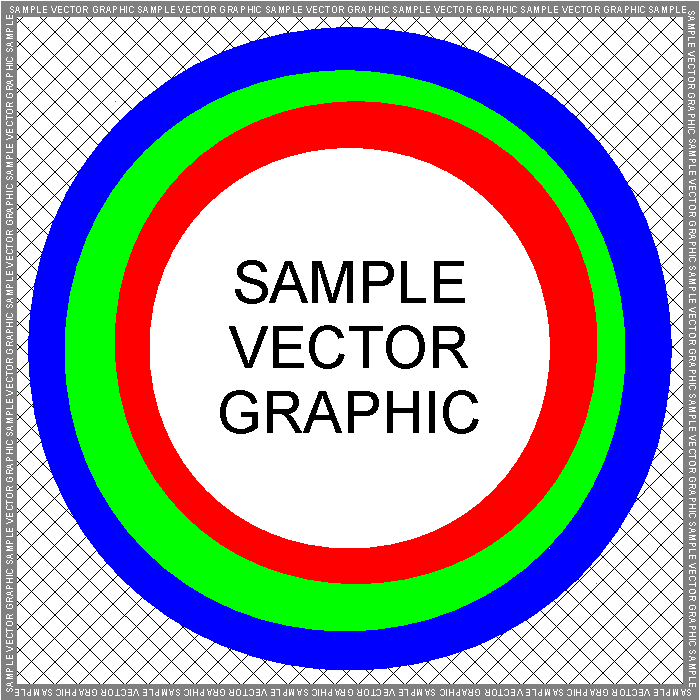
\includegraphics[height=15em]
{Figures/Figure-ChapAbbr-FigureExampleA}
\caption[Insert an abbreviated caption here to show in the List of Figures (optional)]
{Insert the full caption here for this floating figure.}
\label{Figure:ChapAbbr:FigureExampleA}
\end{figure}
%%%%%%%%%%%%%%%%%%%%%%%%%%%%%%%%%%%%%%%%%%%%%%%%%%%%%%%%%%%%%%%%%

This is a reference to \Figure~\fref{Figure:ChapAbbr:FigureExampleA}.
\lipsum[8]

%%%%%%%%%%%%%%%%%%%%%%%%%%%%%%%%%%%%%%%%%%%%%%%%%%%%%%%%%%%%%%%%%
% FIGURE: CHAPABBR: FIGURE EXAMPLE B
\begin{sidewaysfigure*}
\centering\CaptionFontSize
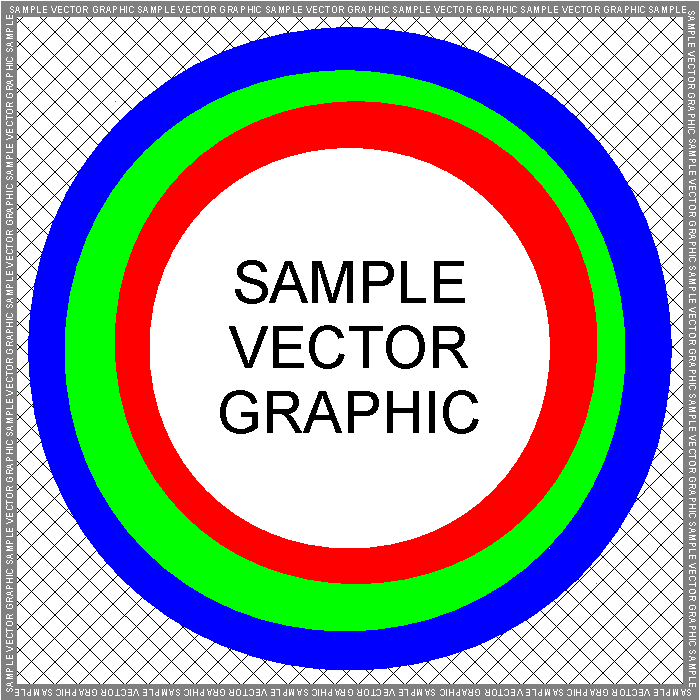
\includegraphics[height=30em]
{Figures/Figure-ChapAbbr-FigureExampleB}
\caption[Insert an abbreviated caption here to show in the List of Figures (optional)]
{Insert the full caption here for this floating figure.
The caption should provide sufficient context to interpret the figure.
Lorem ipsum dolor sit amet, consectetuer adipiscing elit.
Ut purus elit, vestibulum ut, placerat ac, adipiscing vitae, felis.
Curabitur dictum gravida mauris.}
\label{Figure:ChapAbbr:FigureExampleB}
\end{sidewaysfigure*}
%%%%%%%%%%%%%%%%%%%%%%%%%%%%%%%%%%%%%%%%%%%%%%%%%%%%%%%%%%%%%%%%%

Here we say something about \Figures~\fref{Figure:ChapAbbr:FigureExampleA} and~\fref{Figure:ChapAbbr:FigureExampleB}.
Note how the effect in \Figure~\fref{Figure:ChapAbbr:FigureExampleB} is stronger that in \Figure~\fref{Figure:ChapAbbr:FigureExampleA}.
\lipsum[9]

%%%%%%%%%%%%%%%%%%%%%%%%%%%%%%%%%%%%%%%%%%%%%%%%%%%%%%%%%%%%%%%%%
% TABLE: CHAPABBR: EXAMPLE A
\begin{table}
\caption[Insert an abbreviated caption here to show in the List of Tables (optional)]
{Insert the full caption here for this floating table.}
\label{Table:ChapAbbr:TableExampleA}
\centering\CaptionFontSize
\begin{tabular}{c@{\hspace{1em}}l}
\toprule
Symbol & Definition
\\
\midrule
$\alpha$ & insert definition of $\alpha$ here, $\alpha\geq 1$
\\
$\beta$ & insert definition of $\beta$ here, $\beta\geq 2$
\\
$\gamma$ & insert definition of $\gamma$ here, $\gamma\geq 3$
\\
$\delta$ & insert definition of $\delta$ here, $\delta\geq 4$
\\
\bottomrule
\end{tabular}
\end{table}
%%%%%%%%%%%%%%%%%%%%%%%%%%%%%%%%%%%%%%%%%%%%%%%%%%%%%%%%%%%%%%%%%

We summarize our notation in \Table~\tref{Table:ChapAbbr:TableExampleA}.
\lipsum[10]

%%%%%%%%%%%%%%%%%%%%%%%%%%%%%%%%%%%%%%%%%%%%%%%%%%%%%%%%%%%%%%%%%
% TABLE: CHAPABBR: EXAMPLE B
\begin{table}
\caption[Insert an abbreviated caption here to show in the List of Tables (optional)]
{Insert the full caption here for this floating table.
The caption should provide sufficient context to interpret the table.
Lorem ipsum dolor sit amet, consectetuer adipiscing elit.
Ut purus elit, vestibulum ut, placerat ac, adipiscing vitae, felis.
Curabitur dictum gravida mauris.}
\label{Table:ChapAbbr:TableExampleB}
\centering\CaptionFontSize
\begin{tabular}{c@{\hspace{1em}}c@{\hspace{1em}}c}
\toprule
Variable & Initial Value & Value at $t=100$
\\
\midrule
$c$ & $0.012$ & $3.456$
\\
$\delta$ & $0.312$ & $1.416$
\\
$\gamma$ & $0.042$ & $3.252$
\\
$h$ & $0.012$ & $3.353$
\\
$c$ & $0.012$ & $4.446$
\\
$\delta$ & $0.015$ & $3.556$
\\
$\gamma$ & $0.612$ & $6.656$
\\
$h$ & $0.072$ & $7.456$
\\
$c$ & $0.018$ & $8.756$
\\
$\delta$ & $0.912$ & $9.456$
\\
$\gamma$ & $0.092$ & $5.956$
\\
$h$ & $0.012$ & $2.326$
\\
\bottomrule
\end{tabular}
\end{table}
%%%%%%%%%%%%%%%%%%%%%%%%%%%%%%%%%%%%%%%%%%%%%%%%%%%%%%%%%%%%%%%%%

\Table~\tref{Table:ChapAbbr:TableExampleB} summarizes our simulation results.
\lipsum[11]

%%%%%%%%%%%%%%%%%%%%%%%%%%%%%%%%%%%%%%%%%%%%%%%%%%%%%%%%%%%%%%%%%
% TABLE: CHAPABBR: EXAMPLE C (using longtable)
\begin{small}
\begin{longtable}{c@{\hspace{1em}}c@{\hspace{1em}}c@{\hspace{1em}}c}
\caption[Insert an abbreviated caption here to show in the List of Tables (optional)]
{Example of a \texttt{longtable}.
Lorem ipsum dolor sit amet, consectetuer adipiscing elit.
Ut purus elit, vestibulum ut, placerat ac, adipiscing vitae, felis.
Curabitur dictum gravida mauris.}
\label{Table:ChapAbbr:TableExampleC}
\\
\toprule
Index & Variable & Initial Value & Value at $t=100$
\\
\midrule
\endfirsthead
\caption[]{(continued)}
\\
\toprule
Index & Variable & Initial Value & Value at $t=100$
\\
\midrule
\endhead
\endfoot
\bottomrule
\endlastfoot
1 & $c$ & $0.012$ & $3.456$
\\
2 & $\delta$ & $0.312$ & $1.416$
\\
3 & $\gamma$ & $0.042$ & $3.252$
\\
4 & $h$ & $0.012$ & $3.353$
\\
5 & $c$ & $0.012$ & $4.446$
\\
6 & $\delta$ & $0.015$ & $3.556$
\\
7 & $\gamma$ & $0.612$ & $6.656$
\\
8 & $h$ & $0.072$ & $7.456$
\\
9 & $c$ & $0.018$ & $8.756$
\\
10 & $\delta$ & $0.015$ & $3.556$
\\
11 & $\gamma$ & $0.612$ & $6.656$
\\
12 & $h$ & $0.072$ & $7.456$
\\
13 & $c$ & $0.018$ & $8.756$
\\
14 & $\delta$ & $0.912$ & $9.456$
\\
15 & $\gamma$ & $0.092$ & $5.956$
\\
16 & $h$ & $0.012$ & $2.326$
\\
17 & $c$ & $0.012$ & $3.456$
\\
18 & $\delta$ & $0.312$ & $1.416$
\\
19 & $\gamma$ & $0.042$ & $3.252$
\\
20 & $h$ & $0.012$ & $3.353$
\\
21 & $c$ & $0.012$ & $4.446$
\\
22 & $\delta$ & $0.015$ & $3.556$
\\
23 & $\gamma$ & $0.612$ & $6.656$
\\
24 & $h$ & $0.072$ & $7.456$
\\
25 & $c$ & $0.018$ & $8.756$
\\
26 & $\delta$ & $0.912$ & $9.456$
\\
27 & $\gamma$ & $0.092$ & $5.956$
\\
28 & $h$ & $0.012$ & $2.326$
\\
29 & $c$ & $0.012$ & $3.456$
\\
30 & $\delta$ & $0.312$ & $1.416$
\\
31 & $\gamma$ & $0.042$ & $3.252$
\\
32 & $h$ & $0.012$ & $3.353$
\\
33 & $c$ & $0.012$ & $4.446$
\\
34 & $\delta$ & $0.015$ & $3.556$
\\
35 & $\gamma$ & $0.612$ & $6.656$
\\
36 & $h$ & $0.072$ & $7.456$
\\
37 & $c$ & $0.018$ & $8.756$
\\
38 & $\delta$ & $0.912$ & $9.456$
\\
39 & $\gamma$ & $0.092$ & $5.956$
\\
40 & $h$ & $0.012$ & $2.326$
\\
41 & $c$ & $0.012$ & $3.456$
\\
42 & $\delta$ & $0.312$ & $1.416$
\\
43 & $\gamma$ & $0.042$ & $3.252$
\\
44 & $h$ & $0.012$ & $3.353$
\\
45 & $c$ & $0.012$ & $4.446$
\\
46 & $\delta$ & $0.015$ & $3.556$
\\
47 & $\gamma$ & $0.612$ & $6.656$
\\
48 & $h$ & $0.072$ & $7.456$
\\
49 & $c$ & $0.018$ & $8.756$
\\
50 & $\delta$ & $0.912$ & $9.456$
\\
51 & $\gamma$ & $0.092$ & $5.956$
\\
52 & $h$ & $0.012$ & $2.326$
\\
\end{longtable}
\end{small}
%%%%%%%%%%%%%%%%%%%%%%%%%%%%%%%%%%%%%%%%%%%%%%%%%%%%%%%%%%%%%%%%%

\Table~\tref{Table:ChapAbbr:TableExampleC}, which uses a \texttt{longtable}, shows the full details of our simulation.
\lipsum[6]

%%%%%%%%%%%%%%%%%%%%%%%%%%%%%%%%%%%%%%%%%%%%%%%%%%%%%%%%%%%%%%%%%

\subsection{Examples of Enumerated and Itemized Lists}
\label{Section:ChapAbbr:SomeExamples:Lists}

Here are some citations \cite{Examples:Conference03, Examples:Journal03, Examples:Conference04, Examples:Journal04, Examples:Conference05, Examples:Journal05}.
The following is an enumerated list, or numbered list, with multiple levels:

%%%%%%%%%%%%%%%%%%%%%%%%%%%%%%%%%%%%%%%%%%%%%%%%%%%%%%%%%%%%%%%%%
\begin{enumerate}
\item
\label{Item:ChapAbbr:ItemExampleA}
First level item
\item
First level item
\begin{enumerate}
\item
Second level item
\item
Second level item
\begin{enumerate}
\item
Third level item
\begin{enumerate}
\item
Fourth level item
\item
Fourth level item
\end{enumerate}
\item
Third level item
\end{enumerate}
\item
Second level item
\end{enumerate}
\item
\label{Item:ChapAbbr:ItemExampleB}
First level item
\end{enumerate}
%%%%%%%%%%%%%%%%%%%%%%%%%%%%%%%%%%%%%%%%%%%%%%%%%%%%%%%%%%%%%%%%%

We draw your attention to items \ref{Item:ChapAbbr:ItemExampleA} and \ref{Item:ChapAbbr:ItemExampleB} in particular because they are very important in our study.
The following is an itemized list, or unnumbered list, with multiple levels:

%%%%%%%%%%%%%%%%%%%%%%%%%%%%%%%%%%%%%%%%%%%%%%%%%%%%%%%%%%%%%%%%%
\begin{itemize}
\item
First level item
\item
First level item
\begin{itemize}
\item
Second level item
\item
Second level item
\begin{itemize}
\item
Third level item
\begin{itemize}
\item
Fourth level item
\item
Fourth level item
\end{itemize}
\item
Third level item
\end{itemize}
\item
Second level item
\end{itemize}
\item
First level item
\end{itemize}
%%%%%%%%%%%%%%%%%%%%%%%%%%%%%%%%%%%%%%%%%%%%%%%%%%%%%%%%%%%%%%%%%

%%%%%%%%%%%%%%%%%%%%%%%%%%%%%%%%%%%%%%%%%%%%%%%%%%%%%%%%%%%%%%%%%
%%%%%%%%%%%%%%%%%%%%%%%%%%%%%%%%%%%%%%%%%%%%%%%%%%%%%%%%%%%%%%%%%
%%%%%%%%%%%%%%%%%%%%%%%%%%%%%%%%%%%%%%%%%%%%%%%%%%%%%%%%%%%%%%%%%

\section{Some More Examples}
\label{Section:ChapAbbr:SomeMoreExamples}

According to~\cite{IEEEexample:book_typical}, this behavior can be explained this way.
\lipsum[12]

%%%%%%%%%%%%%%%%%%%%%%%%%%%%%%%%%%%%%%%%%%%%%%%%%%%%%%%%%%%%%%%%%
%%%%%%%%%%%%%%%%%%%%%%%%%%%%%%%%%%%%%%%%%%%%%%%%%%%%%%%%%%%%%%%%%
%%%%%%%%%%%%%%%%%%%%%%%%%%%%%%%%%%%%%%%%%%%%%%%%%%%%%%%%%%%%%%%%%

\subsection{Examples of Mathematical Expressions, Definitions, and Theorems}
\label{Section:ChapAbbr:SomeMoreExamples:Math}

We have the following unnumbered mathematical equation:
\[
E=mc^2.
\]
On the other hand, the following is a numbered mathematical inequality:
%%%%%%%%%%%%%%%%%%%%%%%%%%%%%%%%%%%%%%%%%%%%%%%%%%%%%%%%%%%%%%%%%
\begin{align}
x \leq
\frac{\displaystyle\sum_{i=1}^{n} y^2 \cdot \one{y > 1}}
{\displaystyle\int_{-\infty}^{\infty} x^3 \;\text{d}z \cdot
\binom{\alpha}{\beta} \frac{\floor{\frac{a}{b}}}{\ceil{\frac{c}{d}}}}.
\label{Eq:ChapAbbr:EqExampleA}
\end{align}
%%%%%%%%%%%%%%%%%%%%%%%%%%%%%%%%%%%%%%%%%%%%%%%%%%%%%%%%%%%%%%%%%
Inequality~\eqref{Eq:ChapAbbr:EqExampleA} will be applied multiple times to prove our theorems, in a manner similar to \cite{IEEEexample:article_typical, IEEEexample:conf_typical}.
We now introduce the following definition:

\begin{Thm:Definition}[Name of Term Being Defined]
This is the definition of the term, along with relevant conditions, trivial cases, exceptions, etc.
\end{Thm:Definition}

We can rewrite the result of \cite[Theorem~2.5]{IEEEexample:conf_typical} in the following convenient form for our problem:

%%%%%%%%%%%%%%%%%%%%%%%%%%%%%%%%%%%%%%%%%%%%%%%%%%%%%%%%%%%%%%%%%
\begin{Thm:Proposition}
For all \mbox{$a,b,c\in\ZZ^+$}, we have
\label{Thm:Proposition:ChapAbbr:PropositionExample}
\[
a^2+b^3\leq c^4.
\]
\end{Thm:Proposition}
%%%%%%%%%%%%%%%%%%%%%%%%%%%%%%%%%%%%%%%%%%%%%%%%%%%%%%%%%%%%%%%%%

Based on our numerical observations, we make the following conjecture about the upper bound:

%%%%%%%%%%%%%%%%%%%%%%%%%%%%%%%%%%%%%%%%%%%%%%%%%%%%%%%%%%%%%%%%%
\begin{Thm:Conjecture}
If \mbox{$x\geq 3$} and \mbox{$0<y<x^2$}, then for all \mbox{$n\in\ZZ^+$},
\[
\sum_{i=1}^{n} x_i
= x_1 + x_2 + \cdots + x_n
\leq T_{\textup{all}}.
\]
\end{Thm:Conjecture}
%%%%%%%%%%%%%%%%%%%%%%%%%%%%%%%%%%%%%%%%%%%%%%%%%%%%%%%%%%%%%%%%%

Here is a lemma that will be quite useful in deriving our results:

%%%%%%%%%%%%%%%%%%%%%%%%%%%%%%%%%%%%%%%%%%%%%%%%%%%%%%%%%%%%%%%%%
\begin{Thm:Lemma}
[Name of Lemma if any]
\label{Thm:Lemma:ChapAbbr:LemmaExampleA}
If \mbox{$x,y,z\in\ZZ^+_0$}, then \mbox{$f(x+y+z) = 1$}.
\end{Thm:Lemma}
%%%%%%%%%%%%%%%%%%%%%%%%%%%%%%%%%%%%%%%%%%%%%%%%%%%%%%%%%%%%%%%%%

Applying \Lemma~\mref{Thm:Lemma:ChapAbbr:LemmaExampleA} to \cite[Theorem~4.2]{IEEEexample:book_typical} produces the following theorem:

%%%%%%%%%%%%%%%%%%%%%%%%%%%%%%%%%%%%%%%%%%%%%%%%%%%%%%%%%%%%%%%%%
\begin{Thm:Theorem}
[Name of Theorem if any]
\label{Thm:Theorem:ChapAbbr:TheoremExample}
If \mbox{$x+y\geq z$}, then
\begin{align*}
\sum_{i=x}^{y} f(i) \leq z.
\end{align*}
\end{Thm:Theorem}
%%%%%%%%%%%%%%%%%%%%%%%%%%%%%%%%%%%%%%%%%%%%%%%%%%%%%%%%%%%%%%%%%

As a special case of \Theorem~\mref{Thm:Theorem:ChapAbbr:TheoremExample}, we have the following corollary:

%%%%%%%%%%%%%%%%%%%%%%%%%%%%%%%%%%%%%%%%%%%%%%%%%%%%%%%%%%%%%%%%%
\begin{Thm:Corollary}
If \mbox{$x=4$} and \mbox{$y=z$}, then \mbox{$\sum_{i=x}^{y} f(i) = 5$}.
\end{Thm:Corollary}
%%%%%%%%%%%%%%%%%%%%%%%%%%%%%%%%%%%%%%%%%%%%%%%%%%%%%%%%%%%%%%%%%

\lipsum[13]

%%%%%%%%%%%%%%%%%%%%%%%%%%%%%%%%%%%%%%%%%%%%%%%%%%%%%%%%%%%%%%%%%
%%%%%%%%%%%%%%%%%%%%%%%%%%%%%%%%%%%%%%%%%%%%%%%%%%%%%%%%%%%%%%%%%
%%%%%%%%%%%%%%%%%%%%%%%%%%%%%%%%%%%%%%%%%%%%%%%%%%%%%%%%%%%%%%%%%

\section{Conclusion and Future Work}
\label{Section:ChapAbbr:Conclusion}

\lipsum[14-15]

%%%%%%%%%%%%%%%%%%%%%%%%%%%%%%%%%%%%%%%%%%%%%%%%%%%%%%%%%%%%%%%%%
%%%%%%%%%%%%%%%%%%%%%%%%%%%%%%%%%%%%%%%%%%%%%%%%%%%%%%%%%%%%%%%%%
%%%%%%%%%%%%%%%%%%%%%%%%%%%%%%%%%%%%%%%%%%%%%%%%%%%%%%%%%%%%%%%%%

\section{Proofs of Theorems}
\label{Section:ChapAbbr:ProofsOfTheorems}

\noindent
{\color{red}%
Remember to manually disable (and re-enable) updates to the table of contents (TOC), using
\[
\verb|\DisableTOCUpdates|
\text{ and }
\verb|\EnableTOCUpdates|,
\]
if you want to omit subsections, tables, figures, etc., from the table of contents.}

%%%%%%%%%%%%%%%%%%%%%%%%%%%%%%%%%%%%%%%%%%%%%%%%%%%%%%%%%%%%%%%%%

\DisableTOCUpdates

%%%%%%%%%%%%%%%%%%%%%%%%%%%%%%%%%%%%%%%%%%%%%%%%%%%%%%%%%%%%%%%%%

\subsection{Proof of Lemma~\ref{Thm:Lemma:ChapAbbr:LemmaExampleA}}

\lipsum[16-17]
\qedmarker

%%%%%%%%%%%%%%%%%%%%%%%%%%%%%%%%%%%%%%%%%%%%%%%%%%%%%%%%%%%%%%%%%

\subsection{Proof of Theorem~\ref{Thm:Theorem:ChapAbbr:TheoremExample}}

\lipsum[18]

The following lemma will be quite useful in deriving the theorem:

%%%%%%%%%%%%%%%%%%%%%%%%%%%%%%%%%%%%%%%%%%%%%%%%%%%%%%%%%%%%%%%%%
\begin{Thm:Lemma}
\label{Thm:Lemma:ChapAbbr:LemmaExampleB}
If \mbox{$a,b,c\in\ZZ$}, then \mbox{$g(a\cdot b\cdot c) \leq -1$}.
\end{Thm:Lemma}
%%%%%%%%%%%%%%%%%%%%%%%%%%%%%%%%%%%%%%%%%%%%%%%%%%%%%%%%%%%%%%%%%

%%%%%%%%%%%%%%%%%%%%%%%%%%%%%%%%%%%%%%%%%%%%%%%%%%%%%%%%%%%%%%%%%

\begin{proof}
[Proof of Lemma~\ref{Thm:Lemma:ChapAbbr:LemmaExampleB}]
\lipsum[19-20]
\end{proof}

%%%%%%%%%%%%%%%%%%%%%%%%%%%%%%%%%%%%%%%%%%%%%%%%%%%%%%%%%%%%%%%%%

\lipsum[21]
Applying \Lemma~\mref{Thm:Lemma:ChapAbbr:LemmaExampleB} yields the following:
%%%%%%%%%%%%%%%%%%%%%%%%%%%%%%%%%%%%%%%%%%%%%%%%%%%%%%%%%%%%%%%%%
\begin{align}
& A + B + C + D + E + F
+ \alpha + \beta + \gamma + \delta + \Gamma
\notag
\\
&\hspace{5em}
\leq
\Omega + \Sigma + \omega + \sigma + \Theta + \theta + \epsilon
+ S + T + U + V + W + X + Y + Z.
\label{Eq:ChapAbbr:EqExampleB}
\end{align}
%%%%%%%%%%%%%%%%%%%%%%%%%%%%%%%%%%%%%%%%%%%%%%%%%%%%%%%%%%%%%%%%%
Finally, the desired result is obtained by substituting \mbox{$A=b$} into \eqref{Eq:ChapAbbr:EqExampleB}.
\qedmarker

%%%%%%%%%%%%%%%%%%%%%%%%%%%%%%%%%%%%%%%%%%%%%%%%%%%%%%%%%%%%%%%%%

\EnableTOCUpdates

%%%%%%%%%%%%%%%%%%%%%%%%%%%%%%%%%%%%%%%%%%%%%%%%%%%%%%%%%%%%%%%%%
%%%%%%%%%%%%%%%%%%%%%%%%%%%%%%%%%%%%%%%%%%%%%%%%%%%%%%%%%%%%%%%%%
%%%%%%%%%%%%%%%%%%%%%%%%%%%%%%%%%%%%%%%%%%%%%%%%%%%%%%%%%%%%%%%%%

\section{Acknowledgment}
\label{Section:ChapAbbr:Acknowledgment}

Insert chapter acknowledgment here.
\lipsum[22]


\chapter{Summary and Future Work}
\label{Section:Summary}

%%%%%%%%%%%%%%%%%%%%%%%%%%%%%%%%%%%%%%%%%%%%%%%%%%%%%%%%%%%%%%%%%
%%%%%%%%%%%%%%%%%%%%%%%%%%%%%%%%%%%%%%%%%%%%%%%%%%%%%%%%%%%%%%%%%
%%%%%%%%%%%%%%%%%%%%%%%%%%%%%%%%%%%%%%%%%%%%%%%%%%%%%%%%%%%%%%%%%

\section{Summary}
\label{Section:Summary:Summary}

\lipsum[1-6]

%%%%%%%%%%%%%%%%%%%%%%%%%%%%%%%%%%%%%%%%%%%%%%%%%%%%%%%%%%%%%%%%%
%%%%%%%%%%%%%%%%%%%%%%%%%%%%%%%%%%%%%%%%%%%%%%%%%%%%%%%%%%%%%%%%%
%%%%%%%%%%%%%%%%%%%%%%%%%%%%%%%%%%%%%%%%%%%%%%%%%%%%%%%%%%%%%%%%%

\section{Future Work}
\label{Section:Summary:FutureWork}

\lipsum[7-12]


% Back-matter:
%   Bibliography
%   Curriculum Vitae
%   ScholarWorks Agreement
%%%%%%%%%%%%%%%%%%%%%%%%%%%%%%%%%%%%%%%%%%%%%%%%%%%%%%%%%%%%%%%%%
%%                                                       GLOSSARY
%%%%%%%%%%%%%%%%%%%%%%%%%%%%%%%%%%%%%%%%%%%%%%%%%%%%%%%%%%%%%%%%%

\ifPrintGlossary
    \glossarystyle{list}
    \printglossaries
\fi

%%%%%%%%%%%%%%%%%%%%%%%%%%%%%%%%%%%%%%%%%%%%%%%%%%%%%%%%%%%%%%%%%
%%                                                  BIBLIOGRAPHY
%%%%%%%%%%%%%%%%%%%%%%%%%%%%%%%%%%%%%%%%%%%%%%%%%%%%%%%%%%%%%%%%%

\clearpage
\phantomsection
\addcontentsline{toc}{chapter}{Bibliography}

% TODO: improve bibtex settings, maybe move to biblatex. Currently invoking bibtex via the command
%       line, but want to change some settings. (E.g., include URL and DOI hyperlinks.)
% See https://tex.stackexchange.com/questions/3587/how-can-i-use-bibtex-to-cite-a-web-page
\bibliographystyle{\Bibstyle}
\ifx\Bibsettings\empty
    \bibliography{\Bibsettings,Thesis}
\else
    \bibliography{Thesis}
\fi

%%%%%%%%%%%%%%%%%%%%%%%%%%%%%%%%%%%%%%%%%%%%%%%%%%%%%%%%%%%%%%%%%
%%                                              CURRICULUM VITAE
%%%%%%%%%%%%%%%%%%%%%%%%%%%%%%%%%%%%%%%%%%%%%%%%%%%%%%%%%%%%%%%%%

\ifHasCurriculumVitae
    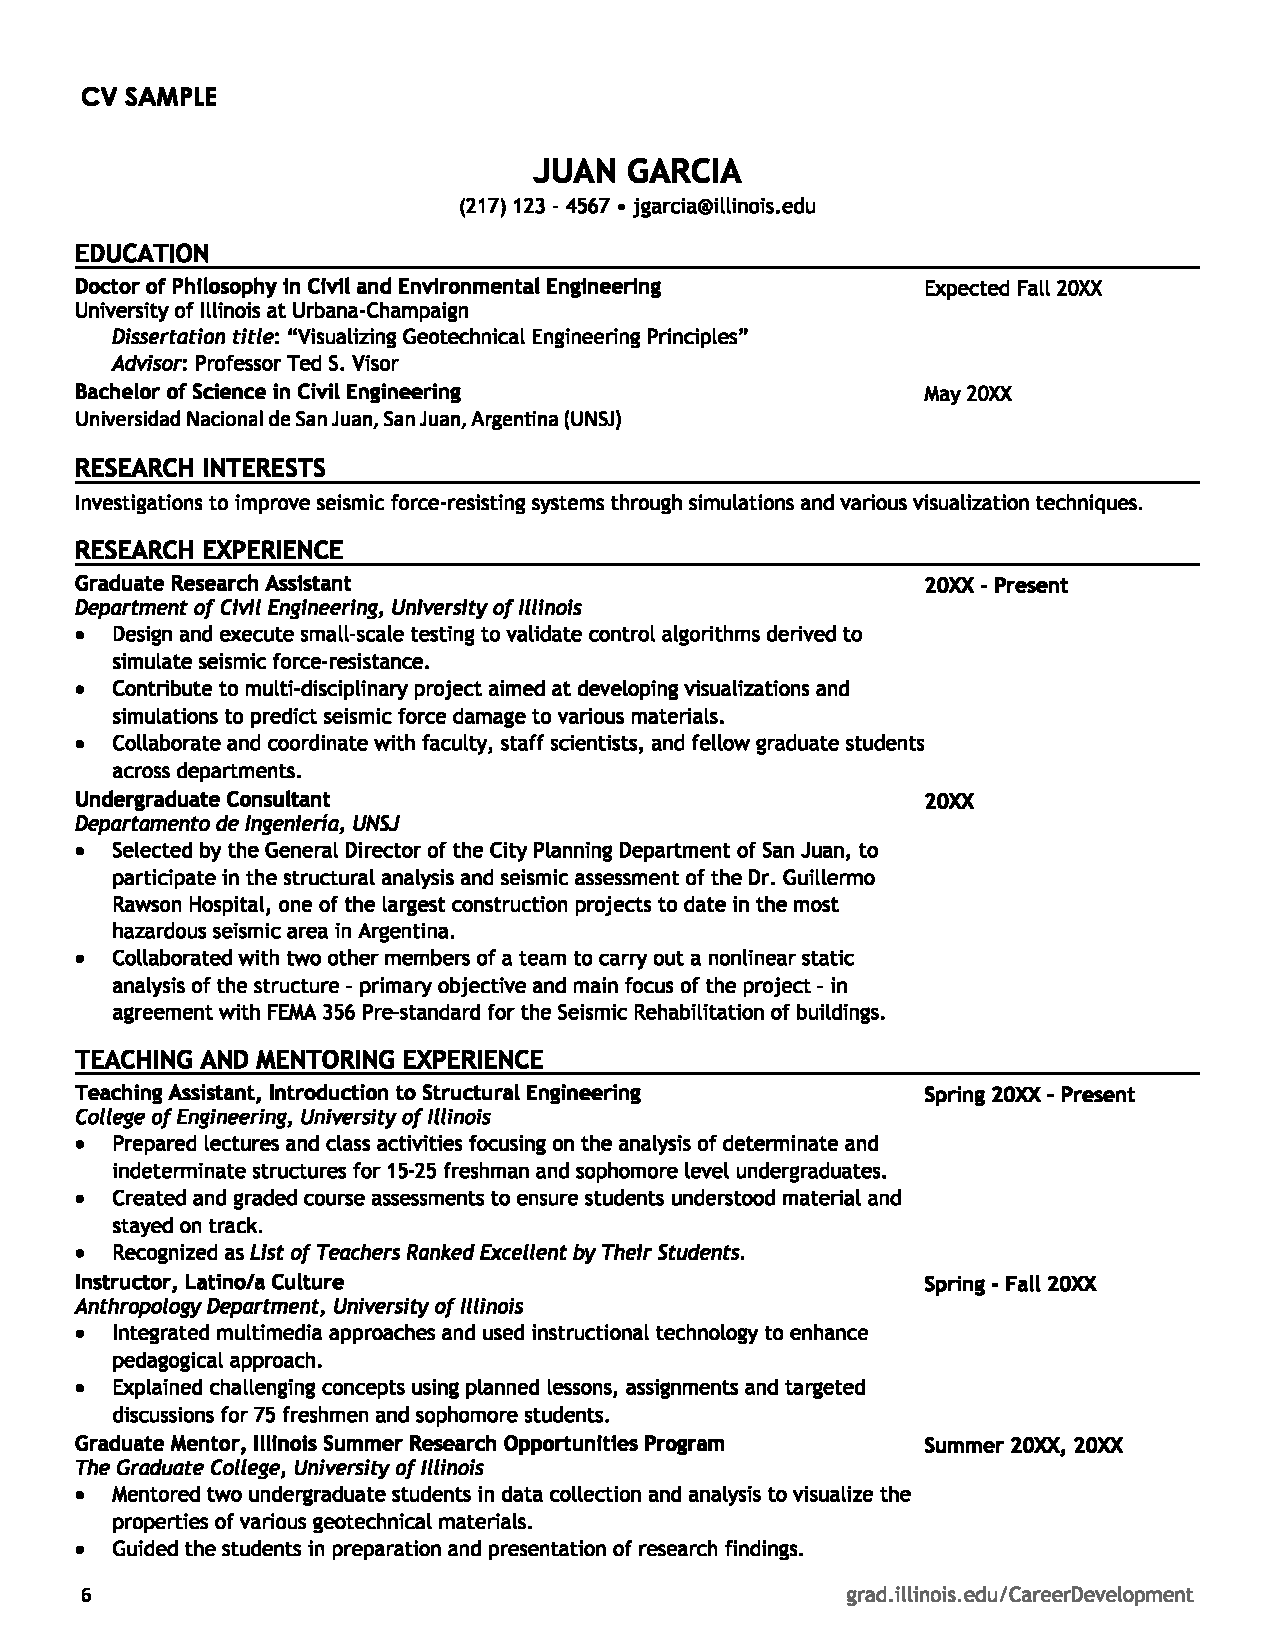
\includepdf[pages=-,pagecommand={\thispagestyle{plain}}]{Forms/CurriculumVitae.pdf}
\fi

%%%%%%%%%%%%%%%%%%%%%%%%%%%%%%%%%%%%%%%%%%%%%%%%%%%%%%%%%%%%%%%%%
%%                                        SCHOLARWORKS AGREEMENT
%%%%%%%%%%%%%%%%%%%%%%%%%%%%%%%%%%%%%%%%%%%%%%%%%%%%%%%%%%%%%%%%%

\ifIncludeForms
    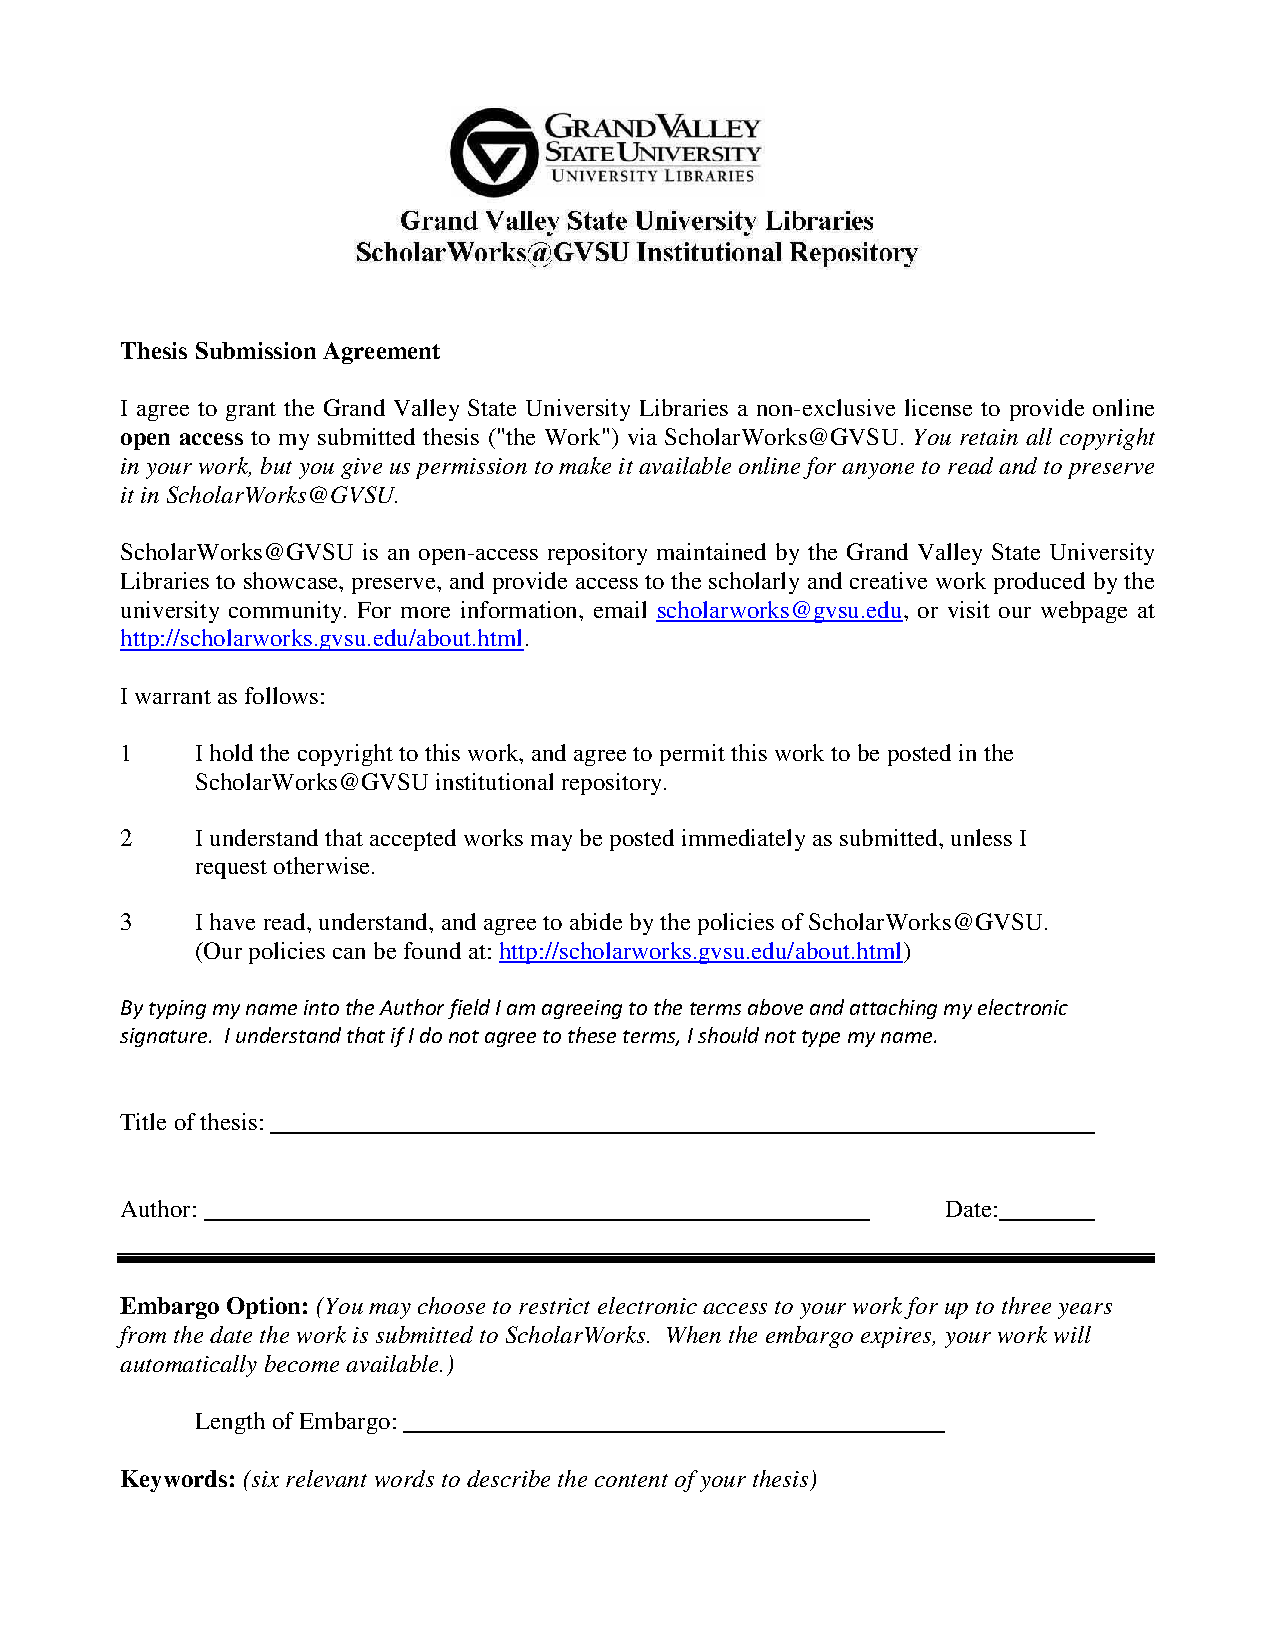
\includepdf{Forms/ScholarWorksAgreement.pdf}
\fi


\end{document}
